\documentclass{article}
\usepackage[utf8]{inputenc}
\usepackage{hyperref}
\usepackage{mathtools}
\usepackage{bbm}
\usepackage{amsfonts}
\PassOptionsToPackage{hyphens}{url}\usepackage{hyperref}

\title{Janka}
\author{Rashad Al-Haddad}
\date{February 2023}

\begin{document}

\maketitle

\begin{abstract}
   Janka is a new DAO managed DeFi primitive serving as a signal adaptor for credit risk assessment, trust, and reputation. Built with Gelato, with code hosted on IPFS, fueled with data from the Graph Protocol, Janka ranks pseudonymous entities by measuring their propensity to repay borrowed assets. Janka enables DeFi lenders, or any entity needed to make an assessment about a pseudonymous entity's trust \& creditworthiness, a reasonable way to see thru the noise in a decentralized and transparent manner.
\end{abstract}

\section{Introduction}
    Web3 credit \& trust scoring is not a new problem, but is one that desperately needs a solution. Capital efficiency in DeFi is incredibly low from loans needing to be highly overcollateralized due to a lack of legal recourse on default. For example, even when assets are highly correlated, the highest liquidation threshold for a loan on AAVE is 80$\%$ LTV\footnote{https://docs.aave.com/risk/asset-risk/risk-parameters}. 
    
    Many new protocols have emerged over the last 2 years offering Web3 credits scores. These protocols have attempted to solve this problem by mining data from the Graph Protocol and using it to power machine learning models hosted on cloud services such as AWS or GCP, which then link to credit risk oracles that provide "on-chain credit scores" for borrowers. These scores tend to be closely kept secrets by these firms, and are not available for public scrutiny or audit. As a result, any DeFi protocol or lender wishing to adopt these scores is required, for the most part, to take these firms at their word. This presents a clear challenge for any DeFi protocol wishing to adopt these scores, especially in the post FTX era, as communities are not likely to desire passing any governance proposals that not only rely on blind trust of opaque models, but also increase their community's dependency on centralized services. As a consequence of this, the DeFi community, both participants and protocols, have been forced to remain stuck with lower levels of capital efficiency, making DeFi less attractive and limiting the growth of liquidity in the ecosystem. 

    To enable new growth for DeFi ecosystem, it is essential for the community to find new solutions for improving capital efficiency. In this paper, we propose Janka, and in particular, the Janka Score as a decentralized solution to credit scoring. Janka is designed to be community managed, community maintained, and fully transparent. Powered by the relatively simple but powerful mathematics behind Bayesian inference, Janka is able to provide solutions for measuring borrower trust and creditworthiness.

\section{How do we decentralize credit?}
To solve this problem, we can begin with first principles. Fundamentally, what does a credit scoring system need to do?

\begin{enumerate}
    \item Monitor and collect events \& transactions
    \item Measure the risk associated with those events
    \item Report some aggregated measure of the risk of those collected events
\end{enumerate}

In particular, a decentralized system will perform (1)-(3) in a way that does not rely on a centralized system (e.g., AWS or GCP), and does so it a way that allows users to prove their score was computed in an honest and valid way to other users without having to rely on centralized intermediary to confirm this was done properly.

While existing Web3 Credit Scores for the most part have not chosen to tackle the problems of (1)-(3) in a decentralized way (and in particular (2)), we propose a unique solution by combining Gelato, The Graph Protocol, and IPFS to run a bayesian inference inspired scoring algorithm, secured with Optimistic Attestation.

\subsection{Architecture for Decentralizing Scoring}
To address (1)-(3), Janka relies on a combination of the Graph Protocol and the Gelato network. The Graph Protocol is a decentralized indexing service that can be used to quickly collect, monitor, and parse on-chain activity pertaining to various contracts and protocols (E.g., AAVE, Compound, Maker, etc). Gelato, meanwhile, acts as a decentralized backend, enabling off-chain computations to be triggered from on-chain events. 

A key problem faced in computing credit scores on-chain is verifying that the computations were performed correctly because contracts have a limited ability to query for historical information. We refer to this problem as the introspection problem \footnote{\url{https://twitter.com/jankascore/status/1628152778920181766?s=20}}. To solve this, Janka relies on the Optimistic Attestation Model. This is the key to what makes our architecture secure in a decentralized way.

Optimistic Attestation is a security model whose security relies on an ecosystem of actors containing at least one honest actor. Janka uses Optimistic Attestation to ensure that off chain calculations of credit scores are done in an honest way. This works as follows:

\begin{enumerate}
    \item To begin, a user loads a dApp in their browser.  
    \item Next, the dApp queries IPFS for the most recent version of the Janka scoring model.
    \item Using data obtained from The Graph Protocol, the scoring model generates a score between 0-100 representing the user's on-chain activity.
    \item The user then submits this score to the Janka Protocol contract function as an attestation, additionally providing a sufficient amount of at-risk Ether as a disincentive for making a fraudulent attestation. To be explicit, it's the user's responsibility for supplying the gas cost of making the attestation.
    \item Once the on-chain attestation is received, an event is emitted which is then received by a verification process running on Gelato Web3 Functions. This verification process runs the very same scoring model and compares the score to what the user attested to, looking for fraudulent claims.
    \item In the cases where an honest user has submitted an accurate attestation, the verification process performs a "no-op" operation and does nothing.
    \item If, however, the verifier determines an attestation is fraudulent, it issues a challenge to the attestation with the correct score, rendering the original attestation invalid. The verifier also claims the attester's at-risk Ether as a penalty for bad behavior. While issuing an on-chain challenge does require the verifier to fund that operation with gas, the expectation is that the verifier should receive more Ether as a result than was spent.
    \item Finally, if a user's attestation has not been challenged within the challenge period, their able to withdraw their at-risk Ether at any point after. Once this at-risk Ether has been withdrawn, the attestation is unable to be challenged.
\end{enumerate}

In this way, the score is computed twice in a sort of confirm then verify fashion, but by requiring the user to post collateral and by further securing the score with optimistic attestation, the score is made further robust to dishonest attestation. Validators on the network will have opportunities to earn bounties by disproving the score, incentivizing honest attestation. 

By hosting our code on IPFS, running off chain computations on a decentralized network like Gelato, and securing it all with Optimistic Attestations, Janka is able to achieve decentralized credit scoring.

\subsubsection{Challenge Proofs}

Once a user has been assigned a Janka score, it's persisted on-chain using an "optimistic" process. For the purposes of illustration, let's assume that a user receives a score of 70 based on their on-chain activity. This user would then submit an attestation to a function exposed by the Janka Protocol smart contract, including: the score, the version of the scoring algorithm used, and the point in time at which the score was generated so that additional on-chain activity occurring at a later point in time doesn't render the score invalid. Importantly, as part of this user's attestation, they're required to provide a sufficient amount of at-risk Ether to discourage fraudulent behavior.

Continuing with our example, once the attestation has been submitted on-chain, a "challenge window" begins. In the current implementation, we have it set to be a fixed number of hours (2 hours in ETH Denver submission), but future implementations we may make this dynamic. In the background, trusted off-chain "verifier" processes continually monitor on-chain activity and, using the same algorithm version, separately compute the very same Janka score and compare it to what the user attested to. If the score matches, the verification process performs a "no-op" operation and continues processing on-chain events; in the situation where the user has made a fraudulent attestation however, the verification process renders the attestation invalid and claims the user's at-risk Ether as a penalty for fraudulent behavior.

In future implementations of the protocol, in order to eliminate centralization risk and trust assumptions, allow-listed verifiers may be augmented by or replaced with an oracle network or zero-knowledge proof techniques. In the present form, the allowlist of trusted verifiers comes from wallets pertaining to Gelato Web3 Function which host our scoring function and invoke the challenge process when a fraudulent score is observed.

\section{How do we Score people?}

    The Janka Score is based on the the principal of Bayesian Inference. It starts out by making an initial assumption, represented by a set of set parameters, about an entity when they come into existence, then allowing the behavior of that entity to migrate the score over a period of time. This migration is driven by an increment function that takes an input about an event regarding the borrower, and outputs an increment to a set of state parameters that describe that borrower. These state parameters can then be used to parameterize a probability distribution, that can be used to ask questions about how likely the borrower is to do something; e.g. repay borrowed capital. 

    \subsection{Getting a Probability -- The JPM}

    The Janka Probability Model, referred herein as the JPM, refers to the linkage between the underlying Beta Distribution, and Increment Function that makes it possible for Janka to produce a probability estimate regarding default risk for an entity. The JPM uses a series of increment functions to guide a modified bayesian inference on the probability of repayment of borrowed capital.

    \subsubsection{Beta Distribution}

    A beta distribution models the likelihood of a Bernoulli Event. A Bernoulli Event is any event that takes a 0, or 1 outcome, such as a coinflip. A beta distribution allows us to ask such questions such as “what is the probability that the probability of observing event ‘x’ is less than p?” In the context of lending this makes a lot of sense. A loan, once issued, can ultimately take an outcome of one of the 2 following types of events “Defaulted” and “Non-Defaulted”. While there are a variety of ways a loan can be kept healthy in the “Non-Defaulted” case (e.g., repayment or deposits of collateral), we are primarily focus on the “Defaulted” state. For most DeFi lending protocols, the “Defaulted” state, is when the loan is fed to the liquidators (example AAVE). Let us represent the “Defaulted” state as a 1, and the “Non-Defaulted” state as a 0. We can now ask the question “what is the probability that the probability of observing event ‘1’ is less than p”. Now we can phrase the Default Risk “p” in terms of a beta distribution.


    A Beta Distribution is rather simple in formation\footnote{"https://en.wikipedia.org/wiki/Beta\_distribution"}. Fundamentally it takes 2 parameters: $\alpha, \beta$. Here “$\alpha$” can represent positive or “good” credit risk, and “$\beta$” can represent bad credit risk. This gives us some useful properties
    \begin{enumerate}
        \item We can represent the expected non-default risk of a borrower as $p=\frac{\alpha}{\alpha+\beta}$
        \item We can represent the variance around that estimate as $v=\frac{\alpha\beta}{(\alpha+\beta)^2(\alpha+\beta+1)}$
        \item Following a Bernoulli distribution, we can get a confidence interval around that estimate as $[\max{(p-z*\sqrt{v},0)},\min{(p+z*\sqrt{v},1)}]$, where the lower bound gives a conservative estimate of risk, and the upper bound gives an aggressive estimate of risk for some reasonable choice of “z” say “2”\footnote{Assuming variance in the estimate of p is normally distributed, z=2 here would provide a 95\% confidence interval for the range in the estimate of p}.
    \end{enumerate}

The principal of the JPM is to dynamically calibrate a choice of $\alpha$ \& $\beta$ so that the outputted probability estimate “p” is reasonably consistent with a borrowers likelihood to return capital prior to liquidated averaged across a group of similar entities looking forward from the calibration time. To do this, the JPM makes use of a non-standard bayesian inference to create a conservative forward looking estimate of risk, derived historical on-chain events. 

\subsubsection{Increment Function}

The increment function takes an input of events about an entity and outputs a vector of floating point changes to make to the parameters of the beta distribution. This is how new information gets incorporated into the Janka Score.

There are a wide variety of possibilities for how these increment function(s) could work, and we are not going to attempt to list all possible combinations, nor recommend a particular choice of increment function as superior to another particular choice or combination. Instead in this document we propose a particular choice for our initial release which we believe is reasonably flexible in how the score migrates over time, conservative with respect to lending risks in DeFi, and could be voted on and changed by the community. Our proposed increment function for initial release works based on 3 primary loan events “origination”, “repayment”, and “default/liquidation”. We also provide modifications for cases to manage collateral deposits, reduce game-ability thru smaller repayment, and to sufficiently cap $\alpha,\beta$ to prevent the score from becoming to sticky.

\paragraph{Increment on Origination}

On origination, principally, the risk of an entity ought to become elevated. As an entity takes on more debt, their capacity to continue to service new debt falls. This is due to capital, generally speaking, being a finite resource.

To make the score as universal as possible, and agnostic to both the borrower wealth and the borrowed asset, we focus on a penalty based on length of serviced history. Borrowers with a longer history will receive less of a penalty on new origination, while borrowers with a fresher history will receive less of a punishment. We believe this as reasonable for newer borrowers may be more likely inexperienced with managing leveraged positions in DeFi, leading to high rates of liquidations. 

To adjust borrower credit on liquidation, so that assed credit risk becomes worsend, we need to adjust $\beta$. We propose the following functional for this operation:

\begin{equation}
\beta \coloneqq  (\beta + c_0*ln(1 + \frac{\zeta_0}{\alpha+\beta}))
\end{equation}

Here the choice of $\zeta_0$ determines the inflection point where new origination starts having a decreasing penalty on score. The idea is as the sum of $\alpha, \beta$ comes sufficiently large the increment approaches the natural log of $1$, which is 0. This effect can then be amplified by tuning $c_0$. For reasonable choices of $c_0, \zeta_0$ the increment will be bounded between 0,2 for most increments. 

When the borrower is new this increment will be much larger, harming their score. This makes sense as a new borrower with a lack of history should naturally be treated with a greater degree of skepticism due to inexperience with servicing debt as compared to a borrower with more established history when taking on more debt.

\paragraph{Increment on Repayment}

Repayment will have the effect of improving the borrowers score. To improve the borrowers score, we need to increment $\alpha$. Here we propose the following conservative estimate to how this could be done:

\begin{equation}
\alpha \coloneqq (\alpha + c_1*ln(1 + \frac{\zeta_1}{\alpha+\beta}))
\end{equation}

Similar to the origination case, as the sum crosses the inflection point determined by $\zeta_1$ the increment slows down. The term $c_1$can be used to amplify or dampen the effect. The idea here is that earlier on as the borrower repays capital their score should improve, but as time goes on these increments should get less and less.

\subsubsection{50\% rule}
As a way to reduce game-ability by structuring repayments into infinitesimally small amounts, we propose the benefit on repayment should follow the 50\% rule. This works as follows :
\begin{enumerate}
    \item If the size of the repayment, in units of the borrowed asset is greater than or equal to 50\% of this size of the outstanding debt, then the call to "\_inc\_repay()"\footnote{\url{https://github.com/jankascore/typescript-scoring/blob/df61ecfc79dda9c751b1e0e713b6c6460fcbc8b5/src/tools/obligor.ts\#L156}} should be made.
    \item Otherwise, award no benefit.
\end{enumerate}

We admit, depending on the degree of token divisibility, that transactions could still be structured into nearly infinitesimally small amounts until the smallest unit of repayment allowed by the borrowed token's decimal's is reached. To prevent this type of game-ability, any protocol adopting Janka Score should consider implementing a minimum repayment size.

\subsubsection{Increment on Deposit}
For most DeFi lending protocols, adding deposits is a way of keeping the loan healthy by reducing the chance of experiencing a liquidation due to insufficient collateralization per a Lending protocol's LTV requirements. A borrower's borrowing limit is effectively set by these liquidation LTV's. Thus adding deposits, can be viewed as both a form of reducing utilization. As reducing outstanding debt by returning the borrowed asset, without withdraw of collateral, serves the same effect, we can view this a synthetic way of repaying debt. Because of this, we choose to provide borrowers with a benefit on deposit.

Following a similar pattern to the 50\% rule (see above), when the borrower makes a collateral deposit that is at least 50\% of the current outstanding collateral value on deposit, we give the repayment benefit.\footnote{\url{https://github.com/jankascore/typescript-scoring/blob/df61ecfc79dda9c751b1e0e713b6c6460fcbc8b5/src/tools/obligor.ts\#L219}}

Admittedly, in the current implementation this could be gamed by structuring collateral deposits across multiple collateral assets supported by the particular lending protocol. In a future version, we hope to make this comparison the value of total outstanding collateral accross all assets on deposit. But note-ably even by structuring deposits, this still ultimately reduces collateral risk, at the cost of gas fees to the borrower. Not to mention, the cost in new collateral to put on deposit grows per deposit of supported collateral assets. So while this is a potential vector to score gaming, it can not be done so cheaply.

\paragraph{Increment on Default / Liquidation}

Naturally default or liquidation should harm a borrowers score. We believe this is reasonable as liquidation demonstrates either a failure of a borrower to return borrowed capital, or a failure of a borrower to monitor the health factor of their positions. To worsen borrower credit, we need to adjust the $\beta$ parameter. Given the cost of liquidations to the ecosystem, being the reason why maintenance LTV's tend to be so high, we propose a relatively sensitive increment function for liquidations

\begin{equation}
\beta \coloneqq (\beta + c_2*ln(1+\frac{\alpha+\beta}{\zeta_2}))
\end{equation}

This function is slightly different in that as the sum grows, the increment logarithmically grows, accelerating beyond the inflection point $\zeta_2$, using $c_2$ to amplify the effect. The reason for this change is to reflect that in absolute terms, default / liquidation is much more costly than repayment. Liquidations are needed in DeFi to prevent loans from being under-collateralized. Lack of legal recourse, and sloppy payers, are the reason why DeFi loans need to be over-collateralized, and relatively capital inefficient. Using liquidation as a proxy for repayment is harmful to the ecosystem. Given the harm this behavior causes, we believe the punishment should be sufficiently harsh. 

\paragraph{Credit Stickiness Function}

We believe that people have a right to have their past behavior forgotten and forgiven over a long period of time. We also believe that prior good behavior from long ago is not necessarily reflective of an entity’s morals, ethics, or propensity to repay at the current point in time. Thus, a good credit score should naturally care more about an entity’s current behavior, rather than something they did long ago. To do this, we are proposing the increment function should be guided by a credit stickiness function. To do this, we can cap the sum of $\alpha,\beta$. Letting $C$ be some cap, we achieve this as follows:

After calling any increment function (origination, repayment, borrow), run the following equations whenever the conditions are true:

\begin{equation}
    \begin{array}{cc}
  \{ & 
    \begin{array}{cc}
      \alpha := \min{(\max{(\alpha - 0.5*(\alpha+\beta-C), 0)}, C)}  & \text{, when } (\alpha + \beta)> C \\
      \beta := \min{(\max{(\beta - 0.5*(\alpha+\beta-C, 0)}, C)}  & \text{, when }(\alpha + \beta)> C
    \end{array}
\end{array}
\end{equation}

Effectively, when the sum is exceeded, we remove half the difference from $\alpha$ and $\beta$, making sure that $\alpha,\beta$ remain strictly non-negative. This has the effect of "forgetting" some old history, allowing the score to continue to migrate without getting stuck in place. 

\subsection{Risks}

The primary risk from a credit perspective in the proposed methodology is that it is agnostic to the the quantity of money borrowed, and as a result the sizing of loans, particularly relative to what a borrower is normally extending, are not reflected in any of the increments. It is Janka's view that we should be a pure measure of credit risk, loan sizing is the resposibility of the lender's underwriter.


Some other risks are as follows

\begin{enumerate}
    \item Miscalibration: As the distribution of factors driving lending risk is likely non-stationary, there is no guarantee that the parameters proposed for the increment function(s) will remain accurate indefinitely, and likely will not. There is also no guarantee that the model as proposed will adjust sufficiently fast to changing credit conditions. Out of sample model performance needs to be carefully monitored, adjusting underlying functions and parameters as market conditions make apparent. 
    \item Gamification: thru structuring repayments and deposits, a borrowers score could become artificially inflated. While this would cost the attacker a lot of gas, the cost of the assets used for structuring, along with some interest, it is not impossible. Thus a lender's underwriter should be careful to measure the median time between repayments, the median time between deposits, the median repayment size, the median borrow size, and the median deposit size to make a holistic decision if this type of fraudulent behavior is present. In a future version of Janka, we will seek to provide decentralized APIs to make some of these statistics readily available.
    \item Exogenous risks: there are many factors not directly related to lending that are not covered in the score that could contribute to a borrowers risk; price volatility comes to mind. Additionally, it is possible that a borrower may be interacting with riskier types of activity such as gambling or trading of niche tokens with thin liquidity. Additionally, Janka score does not capture any risks that may exist due to other addresses the borrower may interact with. Janka scores and other features of 1st order \& 2nd order neighbors ought to be considered to create a more holistic lending decision.
\end{enumerate}

Utimately some risks remain that are not captured with the current implementation of Janka, it remains the lender's responsibility to measure these additional components of risk in order to make a more holistic lending decision.

\subsection{Converting JPM output to Janka Score}

We believe every protocol should be free to decide what scoring scale makes the most sense to them, and as a result plan to offer people the direct ability to make read only calls directly to the JPM at a time post launch. This will enable DeFi protocols to tweak the JPM to fit their needs by potentially re-scoring borrowers based on additional factors, models (be it on or off chain), or context that is specific to a particular protocol. 

Ultimately any protocol wanting the raw $\alpha,\beta$ values could run the scoring script locally themselves to compute it, however at the time of launch, Janka will only store an integer the integer score on chain. The methodology of the integer score is explained in further detail below:

\subsubsection{Methodology}

Recall that a beta distribution can be used to compute the expected value of probability associated with a Bernoulli trial. 

We propose a simple score that would range from 0-100 based on interpreting the probability of an entity not defaulting on a given loan based on the values of $\alpha, \beta$ from the JPM:

\begin{equation}
S = I(100\frac{\alpha}{\alpha + \beta}) + \mathbb{1}\{ I(2\frac{\alpha}{\alpha+\beta}) > 0\}
\end{equation}

Where $1\{\dots\}$ is the indicator function taking a value of 1 when the inequality is true, otherwise 0 when the inequality is not true, and $I(\dots)$ is the integer part of a real number. Effectively, we are multiplying the output probability into 100 to make it into a percentage, then rounding to the nearest whole number.\footnote{In code, this is implemented via a very simple a rounding function. However we expand the mathematical notation here to make it both concise \& clear}

Using this method, the score would very directly translate into an easy to interpret ranking for borrowers. Given a score score of 99, for example, would mean that Janka expects at least a $99\%$ chance that the entity associated that score repays or maintains their debt obligations in line with the loan terms extended. Likewise, a score of 1 would mean a 1$\%$ chance of doing this. This allows the Janka score to be used as a baseline estimator in any DeFi Lenders underwriter, and provides a good starting point for what the creditworthiness of an entity before considering a wider set of features and other mitigating factors.

\subsection{Suggested parameters for launch}

To come up with a reasonable choice of parameters for launch, we ran a simulation to see how the credit score of a new borrower would migrate under a reasonable set of assumptions.

The fitting procedure can be thought as finding as set of model parameters, such that in a controlled environment, the Janka Score will converge reasonably well to a target probability. 

At a high level, we are simulating the path of a single collateral asset, following a GBM, for which in each time period the borrower may borrow against with some random probability $p_b$ 1 unit of a price stable asset (e.g., USDC). In any time period, given the borrower has outstanding debt, they repay 1 unit of the borrowed asset, and withdraw collateral up to the maximum amount allowed by the protocol, guided by maintenance LTV requirements. At each time step, we also consider if the price of the collateral asset would trigger a liquidation. If it does, we assume the bare minimum amount of collateral becomes liquidated, with no liquidation penalty.

Step-by-step, the simulation procedure, works as follows
\begin{enumerate}
    \item Draw a set of random NxM matrices B \& R from a continuous uniform distribution on the domain [0,1], elements i.i.d..
    \item On the B matrix, for each element, assign a value of 1 where the value of the element is > 0.5 else 0.
    \item On the R matrix, assign a value of 1 where the value of the element is > (1 - $p_r$) else 0. 
    \item Generate a random (N, M) matrix and r.v.s. from a standard normal distribution, let's call this Z
    \item Use Z to generate a GBM\footnote{A gentle guide to Geometric Brownian motion can be found here: \url{http://www.mi.uni-koeln.de/wp-znikolic/wp-content/uploads/2017/05/4\_Geometric\_Brownian\_Motion\_28042017.pdf}} with drift r, and terminal time T. Lets refer to this simulated price series as $S$.
    \item Set up (N,M) matrices O, A, B, to track outstanding collateral, alpha, and beta for each borrower at each time step respectively.
    \item Set up a (1,N) collection as an array to guide borrower migration\footnote{this is implemented using a slightly simplified version of our obligor class, written in python \url{https://github.com/jankascore/scoring\_python\_apis/blob/main/refined\_ruleset/src/lib/obligor.py}. Note that the production version differs in order to handle multiple borrows and multiple collateral types. Here we calibrate to a single borrow against a single collateral asset.}
    \item For each of our N borrowers, using the defined methods on the obligor to initiate these actions, at each time step $m\inM$\footnote{We note here that we do not apply the collateral deposit benefit on the optimization. This is because in simulation we add collateral and borrow simultaneously, however a future pass at this procedure may want to look into how this could be integrated.},
    \begin{enumerate}
        \item If $B_{n,m}=1$, draw a loan of size $1$ with collateral $\frac{1}{S_mL_o}$. Add a loan to the obilgor class for borrower n. Note that this will trigger the origination increment function, followed by the stickiness function.
        \item If $R_{n,m}=1$, repay the loan in full and withdraw collateral equal to $\max{(O_{n,m}}, \frac{1}{L_lS_{n,m}})$. Here $O_{n,m}$ refers to the value of the borrower n's outstanding debt at time m. Add this repay using the borrowers add repay function.
        \item Check to see if $\frac{O_{n,m}}{C_{n,m}S_{n,m}} > L_l$, where $C_{n,m}$ is the units of collateral outstanding for borrower $m$ at time $n$, and $L_l$ refers to the liquidation LTV. If the LTV has exceeded the liquidation LTV just , we liquidate just enough collateral to return the borrower's LTV to the liquidated LTV at time m. This amount is $\frac{L_lS_{n,m}C_{m,n} - O_{n,m}}{L_lS_{n,m}-S_{n,m}}$. Pass this repay transaction into the obligor n's "add\_liquidation" method. Note this will trigger the borrowers "inc\_liquidation" and stickiness methods.
        \item Recalling that the above steps will alter the borrowers $\alpha, \beta$ parameters, we store these in matricies $A,B$, $A_{n,m} = \alpha_{n,m}$, and $B_{n,m} = \beta_{n,m}$.
    \end{enumerate}
    \item We compute a matrix P = A / (A + B) by element wise division.
\end{enumerate}

From this $P$ matrix that the simulation procedure gives, we compute the mean ending probability $p = \frac{1}{N}\sum_i^NP_{i,M}$. We seek $c_0,c_1,c_2,c_3,\xi_0,\xi_1,\xi_2$ such that $p \approx _p^*$, holding $C$ at a constant of 200.

To do this, we use a powerful global minimizer called Dual Annealing \footnote{\url{https://docs.scipy.org/doc/scipy/reference/generated/scipy.optimize.dual\_annealing.html}}. Using B, R, and S simulated from above, holding C at a constant of 200, leting $p(\dots)$ indicate the calibrated probabilty in context of all the parameters used to generate it, we minimize the following loss function:
\begin{equation*}
    \mathcal{L}(c_0,c_1,c_2,\xi_0,\xi_1,\xi_2, B, R, S) = (p(B, R, S) - 0.5)^2
\end{equation*}

Here we choose to calibrate at $p^* =0.5$. The idea being that despite liquidations, over time a borrower who repay's 50\% of the time should receive a score of 50. 

We use the following parameters to guide the optimization
\begin{align*}
    N = 1000 \\
    M = 100 \\
    r = 0.04 \\
    \sigma = 0.8 \\
    \Delta_T = \frac{1}{365} \\
    \text{LTV origination} = \frac{1}{1.4} \\
    \text{LTV liq} = \frac{1}{1.2} \\
    p_{repay} = p^* = 0.5
\end{align*}

The result of this optimization is as follows:
\begin{align}
c_0 = 0.24681373 \\  
c_1 = 0.63754091 \\  
c_2 = 0.31491661 \\  
\xi_0 = 124.3596776 \\
\xi_1 = 154.91467195 \\
\xi_2 = 42.90329494 \\
C = 200
\end{align}

We note that the optimizer has selected $c_1 > c_0$ and $\xi_1 > \xi_0$. This ensures in context of liquidations, the score would remain at a stable value of 50 given the borrower repays 50\% of the time. Thus, a borrower who is careful to avoid liquidations, will see there score converge to 100 over a large series of transactions.

To view the juptyer notebook responsible for these results, we reccomend downloading and running the following : \url{https://github.com/jankascore/scoring_python_apis/blob/main/refined\_ruleset/src/notebooks/Fitting%20parameters.ipynb}

\subsection{Example showing converge of score}

To see how the score migrates over time, we can plot the credit migration over each path using the process function from our fitting notebook (see link in above section). Here we simulate the credit score of a borrower, in the context of liquidation risk, with the same parameters as the optimization, with the probability of repayment in any period set to 85\%.

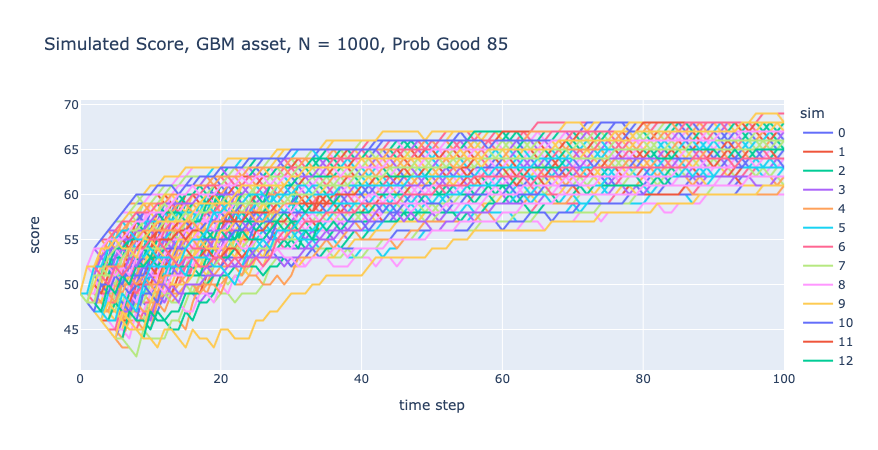
\includegraphics[scale = 0.4]{p85.png}

As we can see, the score improves logarithmically over time, with some variation triggered by either a series of originations with no repayment or liquidation. Although the true probability the borrower repays is roughly 85\%, in context of liquidation, the risk is higher to the lender, and simulating for a collateral asset with 80\% implied vol, seems to suggest an esimated probability of getting capital returned prior to liquidation of somewhere around 65\% after 100 time steps.

We also simulate the downside case with a borrower who has a 15\% chance of returning capital in any period.

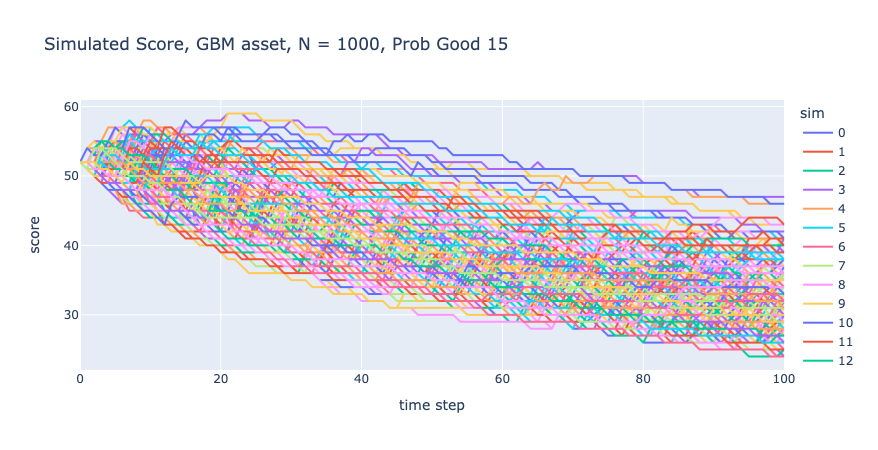
\includegraphics[scale = 0.4]{p15.png}

Here we see the score is lower, but can still see that this is a random process, given that for short periods of time, borrowers with generally risky behavior can still experience credit improvements. On some paths, the score approaches almost 60. On the downside there is certainly more variance, but in general we'd advise lenders to treat anything under 60 as "bad" credit.

We also simulate a scenario where for the first 50 time steps the borrower has an 85\% chance of returning capital, but in every subsequent time step after t = 50 this decreases to 15\%. This let's us simulate how responsive the score is to changing credit conditions.

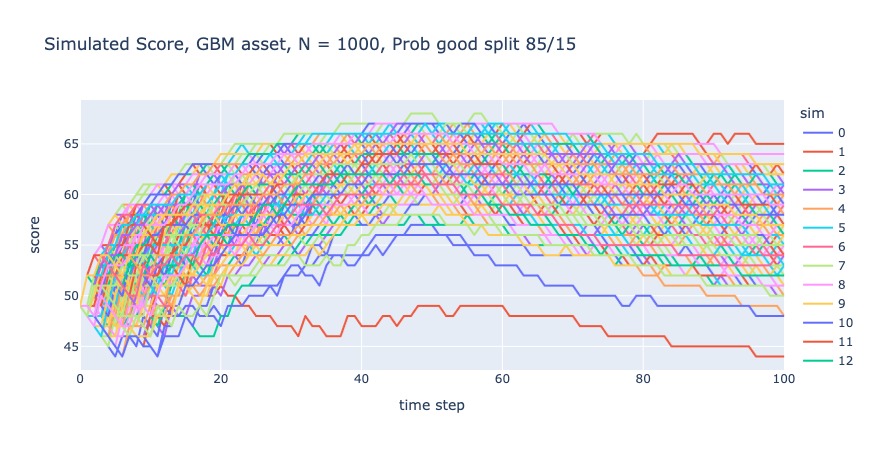
\includegraphics[scale = 0.4]{splitprob.png}

As we can see, there is a very obvious kink around t = 50, and a clear downtrend by t = 60. We recommend lenders to be mindful of how a borrowers score has migrated over a 10 day window to watch for changing credit conditions. 

Ultimately the interpretation of the Janka score in a lending decision should be a holistic decision determined by many factors. However in general, we'd advise the following interpretation
\begin{enumerate}
    \item Scores $\leq$ 60 are bad credit
    \item Scores 61-70 are okay credit
    \item Scores 71-80 are good credit
    \item Scores 81-90 are great credit
    \item Scores 91+ are excellent credit
\end{enumerate}

Generally the lower bound of the confidence interval should be checked as well. For example, a score of 81, with a lower bound of 59 from a 95\% confidence interval should not be treated as great credit.
\section{Applications of Janka Score}
\subsection{Lending}
Janka score very naturally lends itself to lending, as it directly measures the probability of a borrower returning a borrowed sum to a lender. Lenders can use the Janka Score to get a gauge for the probability of liquidation given an appropriately sized LTV at the time of origination. From this, the lender can derive what the cost of financing (the interest rate) should be at the time of origination given the Janka Score and origination LTV given the lender's risk tolerance and how aggressive they want to be in different market states.
\subsubsection{An additional consideration}
We note that Janka Score does not measure the probability of liquidation given a loan of a specific size. This is because the Janka score is trying to measure generic credit risk, rather than making opinions about how a particular loan size may or may not be appropriate for a borrower. Loan sizing is a job for the credit underwriter, and the credit underwriter should be careful to ensure loans are sized appropriately given any posted collateral and the borrowers demonstrated average repay amounts; among all other exogenous factors. Janka Score is the most reliable when the loan is sized given the historical collateral ratios the borrower has borrowed with and the loan is sized appropriately given average borrow and repayment values. The exact sizing of such, Janka ultimately leaves to the lender to decide what is appropriate for them. 
\subsection{Collateralized Trust Obligation}
Extending Janka score beyond the scope of lending requires us to establishing a framework a collateralized trust obligation. 

To understand what this means, let's first consider a concrete example of a simple loan between two friends. Suppose Bob borrows $\$100$ from Alice, with the stipulation that Bob should return the money with 10 days. Bob puts nothing tangible to Alice. Suppose after 10 days passes, Bob does not repay the loan, only providing Alice some lousy excuse. Some more time passes and Bob still does not return the loan. Alice, upset that she has not been repaid, begins to tell her friends, some of which may know Bob or Bob's friends, that Bob has not repaid this loan. Word spreads that Bob owes Alice $\$100$, and as a result people become more reluctant to lend Bob another $\$100$.

In this example, as Bob and Alice were in a community of people who know each other, what Bob put to Alice as collateral was his reputation. As a result of not making good on his promise to repay the loan, Bob's reputation has been harmed, and this may follow him well into the future. While this example may work well in small communities where the lending and borrowing parties may know each other on a first name basis, it does not extend well to a decentralized context, where individuals may exist in distant geographical locations with different laws, regulations, and lack of legal recourse.

To perform the same in DeFi we would replace the promise to repay with the postage of some collateral with monetary value, agreed upon by Bob and Alice (maybe's Bob's prized baseball card collection). If Bob doesn't repay, Alice simply liquidates the collateral. Effectively the promise to repay is now collateralized by the collateral posted by Bob. 

Now, if instead we were to simply replace the promise to repay, with any arbitrary promise (say to mow the lawn, deliver physical goods, return physical items borrowed, etc), then we can think about collateralizing the promise to do something or perform some action in and of itself as a collateralized trust obligation. By abstracting in this way we can now generate a trust score to measure how likely someone is to make good on a promise.

With Janka Score, we could envision people would attest that another address has made a promise to them, and then that address would post collateral to that promise. As long as the promise is kept, the collateral would be returned to the user, and the user would receive a benefit as if they have repaid a loan. Thus as they continue to make good on these obligations, they would see their score improve.

Some possible applications on this could include:
\begin{enumerate}
    \item Lending out physical items, such as books, laptops, and solar panels.
    \item Rentals, such as cars and apartments 
    \item Digital Goods, GameFi, etc.
    \item Accounts receivables, lending against future expected income.
\end{enumerate}


\subsection{Collateralized Reputation Obligation}

It is often the case that members of a reputable organization (such as a large corporate, university, government, etc) become more trustworthy as often their continued membership as a part of these organizations depends on them making good on their promises and commitments.

We envision that by structuring collateralized trust obligations via a guarantority model, we can achieve reputation sharing across the Janka ecosystem.

To envision how this could work, let's think thru an example with a DAO. Let's suppose a we have a sizeable DAO with a large amount of goodwill and reputation within the broader community. Let's further suppose that if the members of the DAO collectively agree to make good on some promise, the broader community for which this DAO is a part of will broadly trust the DAO to make good on said promise. 

Let's suppose Bob is a member of this DAO, and that Bob individually has lower reputation within the broader community, but is generally an honest actor. Suppose Bob wishes to make a promise to do something that requires a large amount of trust, or credit, to be a part of. We envision that reputation from the DAO could be extended to Bob as follows:

\begin{enumerate}
    \item Bob assigns some stake with monetary value to the DAO.
    \item Bob then enters into a promise using the DAO as a guarantor on that promise (the DAO aggrees to furfill the promise if Bob does not).
    \item As long as Bob makes good on the promise, both Bob's and the DAO's Janka scores would improve (see collateralized trust obligation).
\end{enumerate}

In effect, reputation \& credit can be shared via this guarantority model. By putting to the guarantor some collateral and/or potentially a fee, the guarantor allows the individual to utilize their credit score. Thus, we see some practical applications such as:
\begin{enumerate}
    \item Loans. DAOs or other organizations could act as a backstop or insurance to make good on a loan when the individual that borrowed that loan does not. The individual, with the consent of the guarantor, would benefit from the high creditworthiness of the guarantor, allowing access to credit on better terms than they could otherwise get individually.
    \item Rentals. Be it apartments, cars, or other goods (digital or physical) that can be rented out, a common problem is that the creditworthiness of the individual may be insufficient given the liability imposed by the rental contract. Guarantors can share their creditworthiness with the individuals wishing to engage in these agreements, allow them access to rentals that they would otherwise not be able to access.
\end{enumerate}

\section{How do we maintain our score?}
At initial launch, Janka will be entirely governed and maintained by Janka Labs while we work out all the kinks and potential bugs with application and underlying algorithm. However, as Janka is intended to be a community driven public good, our plan is to transition into a DAO governed model as quickly as possible post launch. This will be achieved with the launch of Janka DAO.

\subsection{Janka DAO}

Janka at it's heart is a public good that is maintained by the community. For Janka, the community that maintains the score is Janka DAO. Janka DAO achieves this by having it's members make and vote on proposal for changes in the scoring algorithm. When a proposal is passed, the code that govern's Janka's scoring algorithm will update to be inline with approved proposals.

\subsubsection{Governance}
Governance of Janka DAO is achieved via a combination governance tokens and soul bound NFTs. When Janka DAO launches, users will receive soul bound NFTs when they mint their Janka Score, which will hold their current score. This NFT also represents membership in Janka DAO. As a member of the DAO, users can make proposals, vote for changes, or stake to receive rewards. Voting will follow a quadratic scheme where the number of votes is equal to the sum of the square root of the number of governance tokens staked to a proposal by each user. When a proposal passes, regardless of whether a user is on the winning or losing side of the vote, their governance tokens will become eligible for withdraw.

\subsubsection{Staking}

DAO members will be able to stake their tokens with the DAO in order to receive a share of of protocol revenue. While Janka is a public good, with the launch of the DAO, Janka will charge a very small fee to interact with the scoring contract. These fees will accrue to DAO's treasury, where then DAO members can exchange their DAO tokens for a share of protocol revenue at a fixed percentage pro rata. These exchanged tokens reclaimed by the DAOs treasury are paid out as staking rewards to stakers. 

\subsection{CSRs -- Contract Service Revenue}
Contract Service Revenue is at the core of how Janka protocol generates revenue to support the continued growth and maintenance of the ecosystem. This is done by collecting a small fee on top of the gas fee necessary to interface with the contracts. This fee would be set at the launch of Janka DAO by Janka Labs (in an amount to be determined), and later set by Janka DAO via governance proposals. Fee revenue accumulates to the Janka treasury, where then it can then be exchanged at a fixed percentage to Janka DAO members in exchange for Janka DAO tokens. 

\subsection{Janka Labs}
Janka Labs is intended to be the real world entity that is responsible for implementing governance proposals from the DAO, and broadly ensuring the health of the ecosystem. At initial launch, Janka Labs would be entirely responsible for managing the ecosystem. After a period of time has passed, and Janka Lab's governing members feel the ecosystem is mature enough to begin standing on it's own, control would be ceded to the DAO for long term maintenance and management. At that point, Janka Labs would serve only to implement the will of Janka DAO, and to promote the health and growth of the Janka Ecosystem.

\section{Additional Considerations and Concluding Thoughts}
Credit scores in Web3 are not a new problem. Many companies over the last 2 years have come into the space, focusing primarily on predicting DeFi liquidations with opaque machine learning algorithms hosted on existing web 2 architecture such as AWS \& GCP. As of writing, despite 10's of millions of U.S. Dollars of VC money flowing into these startups, existing DeFi lending protocols have not broadly adopted the scores from these Web3 Credit Bureaus into their products. While there are many possible explanations, it would appear that DeFi protocols are not interested in increasing their dependency on centralized services or non-transparent companies \& individuals; which has become especially relevant in the post FTX era.

Janka Score provides a transparent, simple, and community managed algorithms hosted on IPFS, powered by the Gelato Network and The Graph Protocol. With Janka score, DeFi lending protocols will be able to gauge a user's broad credit risk, enabling them to deliver more favorable lending terms, and increased capital efficiency in the DeFi ecosystem. Long term, we can see Janka Score powering more complex agreements involving trust thru collateralized trust obligations and reputation sharing. 

For DeFi to be successful long term, we will need solutions like Janka score that are able to improve capital efficiency. Currently most DeFi lending products act more like debit cards, which severely limits the amount of money one can borrow thru these systems. Many new primitives will be needed around measuring risk, underwritering, fraud, and identity to bring DeFi to it's full potential. We hope that Janka, or some derivative, will be a part of that long term solution. 

\subsection{Special Thanks}
Special thanks go out to Colin Nielson, for thinking through the high level architecture for optimistic credit attestations, and to Mac Kiminski and Dan Simmons for putting together the architecture that powers Janka Score. Special thanks also go to Daniel Ritchie for his tireless efforts in building Janka's community.

\section{Footnotes Listed}
Footnotes are listed below in the order they appear.
\begin{enumerate}
\item \url{https://docs.aave.com/risk/asset-risk/risk-parameters}
\item \url{https://twitter.com/jankascore/status/1628152778920181766?s=20}
\item \url{"https://en.wikipedia.org/wiki/Beta\_distribution"}
\item Assuming variance in the estimate of p is normally distributed, z=2 here would provide a 95\% confidence interval for the range in the estimate of p
\item \url{https://github.com/jankascore/typescript-scoring/blob/df61ecfc79dda9c751b1e0e713b6c6460fcbc8b5/src/tools/obligor.ts\#L156}
\item \url{https://github.com/jankascore/typescript-scoring/blob/df61ecfc79dda9c751b1e0e713b6c6460fcbc8b5/src/tools/obligor.ts\#L219}
\item In code, this is implemented via a very simple a rounding function. However we expand the mathematical notation here to make it both concise \& clear.
\item A gentle guide to Geometric Brownian motion can be found here: \url{http://www.mi.uni-koeln.de/wp-znikolic/wp-content/uploads/2017/05/4\_Geometric\_Brownian\_Motion\_28042017.pdf}
\item This is implemented using a slightly simplified version of our obligor class, written in python \url{https://github.com/jankascore/scoring\_python\_apis/blob/main/refined\_ruleset/src/lib/obligor.py}. Note that the production version differs in order to handle multiple borrows and multiple collateral types. Here we calibrate to a single borrow against a single collateral asset.
\item We note here that we do not apply the collateral deposit benefit on the optimization. This is because in simulation we add collateral and borrow simultaneously, however a future pass at this procedure may want to look into how this could be integrated.
\item \url{https://docs.scipy.org/doc/scipy/reference/generated/scipy.optimize.dual\_annealing.html}
\end{enumerate}

\end{document}
